%% LaTeX-Beamer template for KIT design
%% by Erik Burger, Christian Hammer
%% title picture by Klaus Krogmann
%%
%% version 2.1
%%
%% mostly compatible to KIT corporate design v2.0
%% http://intranet.kit.edu/gestaltungsrichtlinien.php
%%
%% Problems, bugs and comments to
%% burger@kit.edu

\documentclass[19pt]{beamer}

%% SLIDE FORMAT

% use 'beamerthemekit' for standard 4:3 ratio
% for widescreen slides (16:9), use 'beamerthemekitwide'

\usepackage{templates/beamerthemekit}
\usepackage{wrapfig}
% \usepackage{templates/beamerthemekitwide}

%% TITLE PICTURE

% if a custom picture is to be used on the title page, copy it into the 'logos'
% directory, in the line below, replace 'mypicture' with the 
% filename (without extension) and uncomment the following line
% (picture proportions: 63 : 20 for standard, 169 : 40 for wide
% *.eps format if you use latex+dvips+ps2pdf, 
% *.jpg/*.png/*.pdf if you use pdflatex)
\titleimage{Gruppenarbeit_klein}

%% TITLE LOGO

% for a custom logo on the front page, copy your file into the 'logos'
% directory, insert the filename in the line below and uncomment it

\titlelogo{Logo_IOSB}

% (*.eps format if you use latex+dvips+ps2pdf,
% *.jpg/*.png/*.pdf if you use pdflatex)

%% TikZ INTEGRATION

% use these packages for PCM symbols and UML classes
% \usepackage{templates/tikzkit}
% \usepackage{templates/tikzuml}

% the presentation starts here

\title[PCC]{Privacy Crash Cam:\\ Entwurf}
\subtitle{App, Web-Interface und Web-Dienst}
\author{Giorgio G., Christoph H., David L.,  Josh R.,  Fabian W.}

\institute{Karlsruher Institut f\"ur Technologie, Fraunhofer Institut f\"ur Optronik, Systemtechnik und Bildauswertung}

% Bibliography

\usepackage[citestyle=authoryear,bibstyle=numeric,hyperref,backend=biber]{biblatex}
\addbibresource{templates/example.bib}
\bibhang1em

\begin{document}

% change the following line to "ngerman" for German style date and logos
\selectlanguage{english}

%title page
\begin{frame}
	\titlepage
\end{frame}

\section{Aufgabenstellung}
\subsection{Szenario}
\begin{frame}{Szenario}
	\begin{center}
		%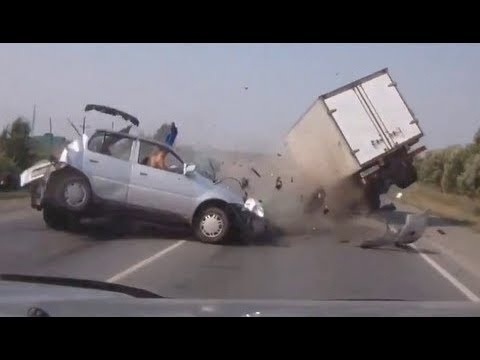
\includegraphics[scale=0.55]{logos/UnfallSzenario} 
		%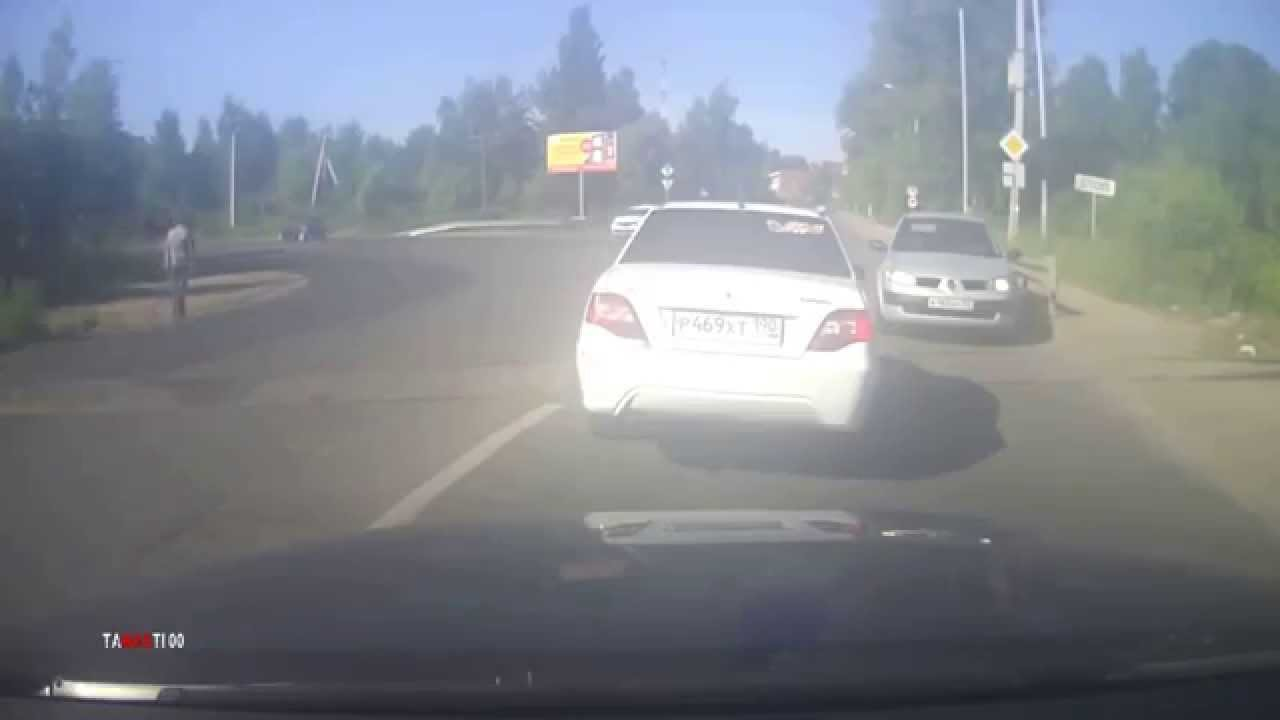
\includegraphics[scale=0.25]{logos/UnfallSzenario2} 
		%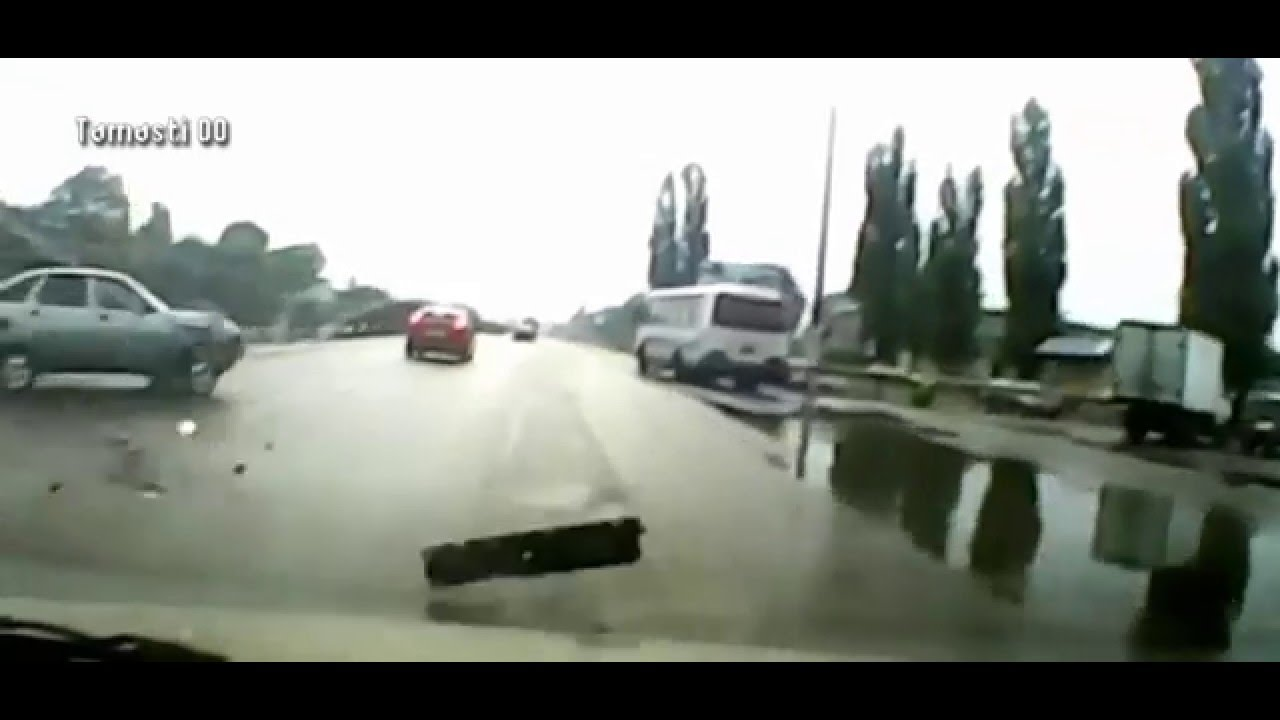
\includegraphics[scale=0.25]{logos/UnfallSzenario3} 
	\end{center}
\end{frame}

\subsection{Aufgabenstellung}
\begin{frame}{Aufgabenstellung}
	\begin{itemize}
		\item Funktionsfähiger Entwurf nach Vorgaben des Pflichtenhefts
		\pause
		\item Aussagekäftige Klassendiagramme
		\pause
		\item Beschreibung der Klassen
	\end{itemize}
\end{frame}

\section{App}
\begin{frame}{App}
  \begin{columns}[T]
    \begin{column}{.5\textwidth}
		\begin{itemize}
    		\item Grundlegendes
			\begin{itemize}
				\item Vertraut machen mit Android API und Designprinzipien
				\item Grundlegender Entwurf durch Anwenden von Entwurfsmustern
				\item Feinschliff durch bessere Strukturierung und Namensgebung
			\end{itemize}
			\item Besondere Probleme
			\begin{itemize}
				\item Ringpuffer
				\item Asynchrone Vorgänge in Android
			\end{itemize}
		\end{itemize}
    \end{column}
  \end{columns}
\end{frame}


\section{Web-Interface}
\begin{frame}{Web-Interface}
  \begin{columns}[T]
    \begin{column}{.5\textwidth}
    		\begin{itemize}
    			\item Grundlegendes
    			\begin{itemize}
					\item Vertraut machen mit Vaadin
					\item Entwerfen Grundlegender Struktur einer Gui
					\item Anzeige und Logik Funktionalität sinnvoll trennen
				\end{itemize}
    			\item Besondere Probleme
    			\begin{itemize}
					\item Kommunikation mit dem Web-Dienst
					\item Entkoppeln von Logik und Anzeige
				\end{itemize}
    		\end{itemize}
    \end{column}
    \begin{column}{.5\textwidth}
    		%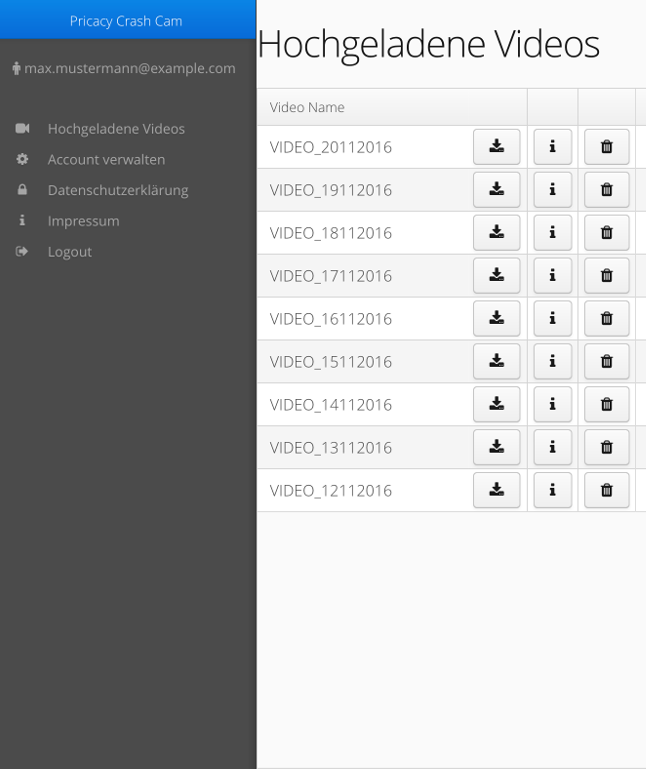
\includegraphics[scale=0.5]{../subtopicsFuncspec/Res/Mockups/Webinterface_small_pres}
    \end{column}
  \end{columns}
\end{frame}

\section{Web-Dienst}
\begin{frame}{Web-Dienst}
	\begin{itemize}
		\item Grundlegendes
			\begin{itemize}
				\item Vertraut machen mit Jetty and Jersey
				\item Rest Anfragen und JSON Objekte
				\item Erstellen eines Grundlegenden Entwurfs
			\end{itemize}
		\pause
		\item Besondere Probleme
			\begin{itemize}
				\item Videoverarbeitung mit per Pipeline
				\item Großer Umfang an Funktionalität
			\end{itemize}
	\end{itemize}
\end{frame}

\section{Organisation}

\subsection{Aufgabenverteilung}
\begin{frame}{Aufgabenverteilung}
  \begin{columns}[T]
    \begin{column}{.5\textwidth}
    		\begin{itemize}
    	\item Christoph H.
			\begin{itemize}
				\item Web-Interface
				\item Präsentation
			\end{itemize}
		\item David L.
			\begin{itemize}
				\item Web-Dienst
			\end{itemize}
		\item Fabian W.
			\begin{itemize}
				\item Web-Dienst
			\end{itemize}
    		\end{itemize}
    \end{column}
    \begin{column}{.5\textwidth}
    \begin{itemize}
		\item Giorgio G.
			\begin{itemize}
				\item App
				\item Präsentation
			\end{itemize}
		\item Josh R.
			\begin{itemize}
				\item App
				\item Web-Dienst
			\end{itemize}
	\end{itemize}
    \end{column}
  \end{columns}
\end{frame}

\subsection{Fazit}
\begin{frame}{Fazit}
   \begin{columns}[T]
    \begin{column}{.5\textwidth}
    		\begin{itemize}
    		\item SCHEIS SCHWER DAS MAL ZU MACHEN
    		\end{itemize}
    \end{column}
   \end{columns}
\end{frame}

\subsection{JIRA}
\begin{frame}[allowframebreaks]{JIRA}
	\begin{figure}
		\begin{center}
			%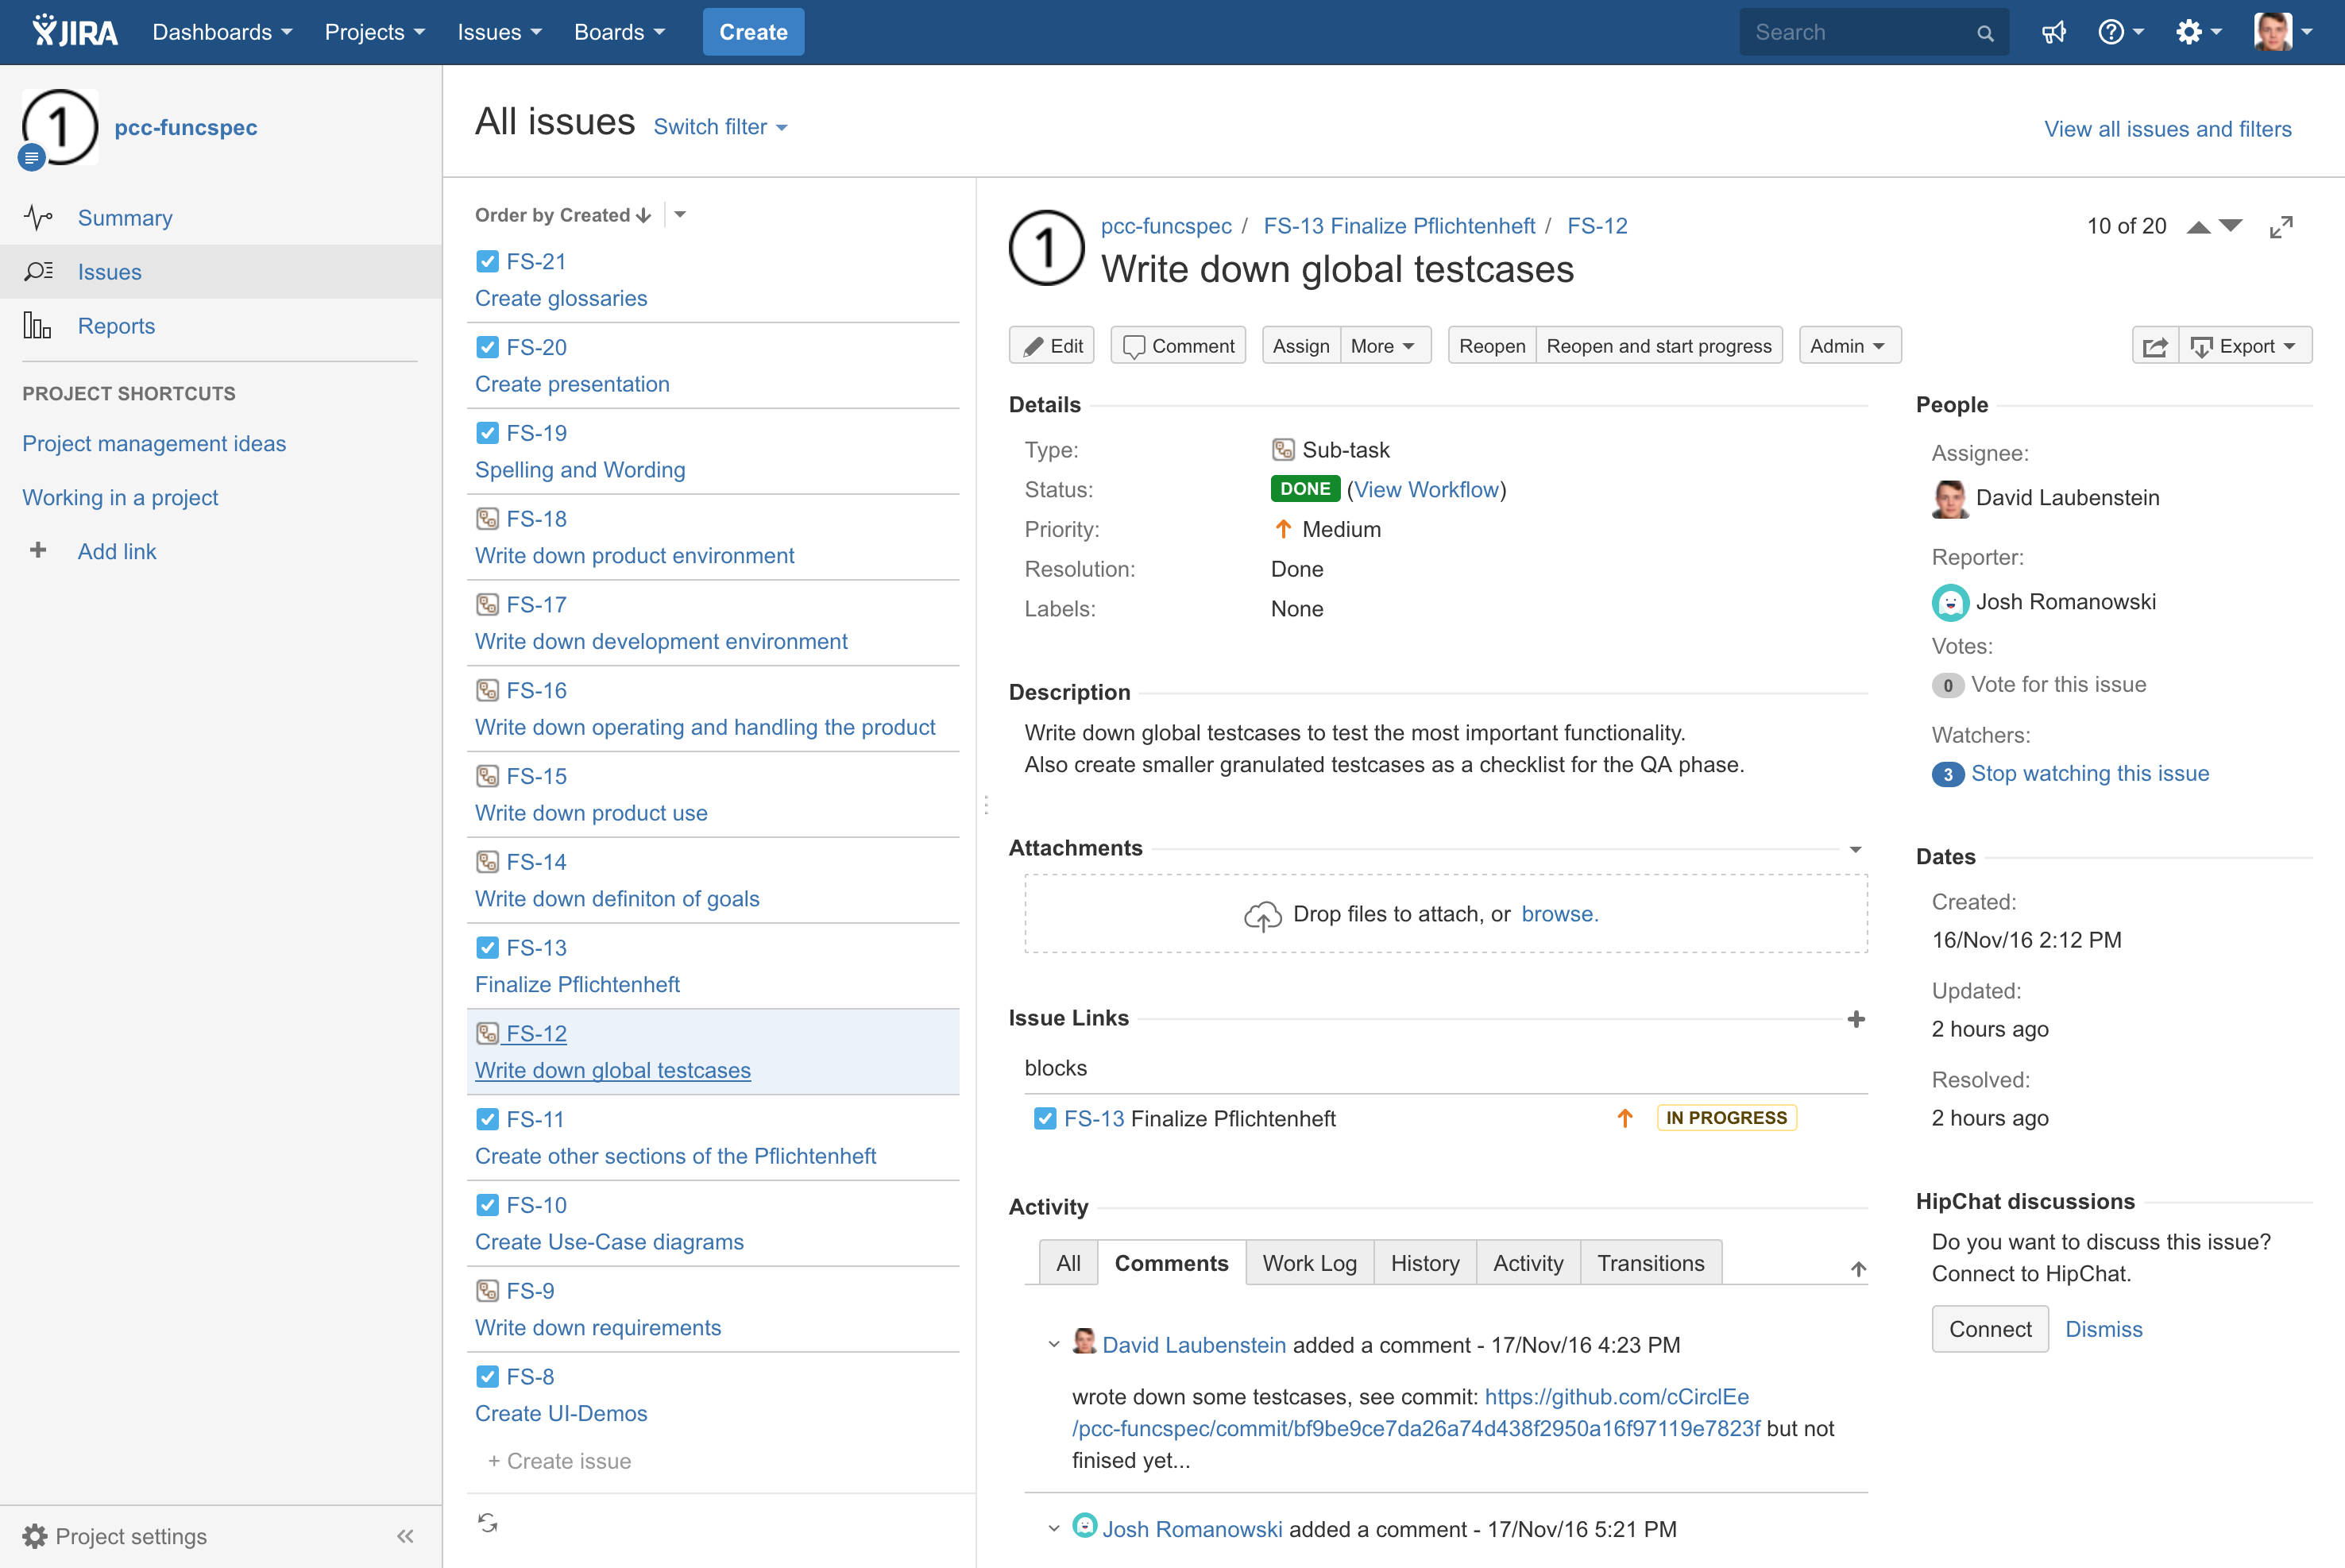
\includegraphics[scale=0.18]{logos/JIRA01} 
		\end{center}
		\framebreak
		\begin{center}
			%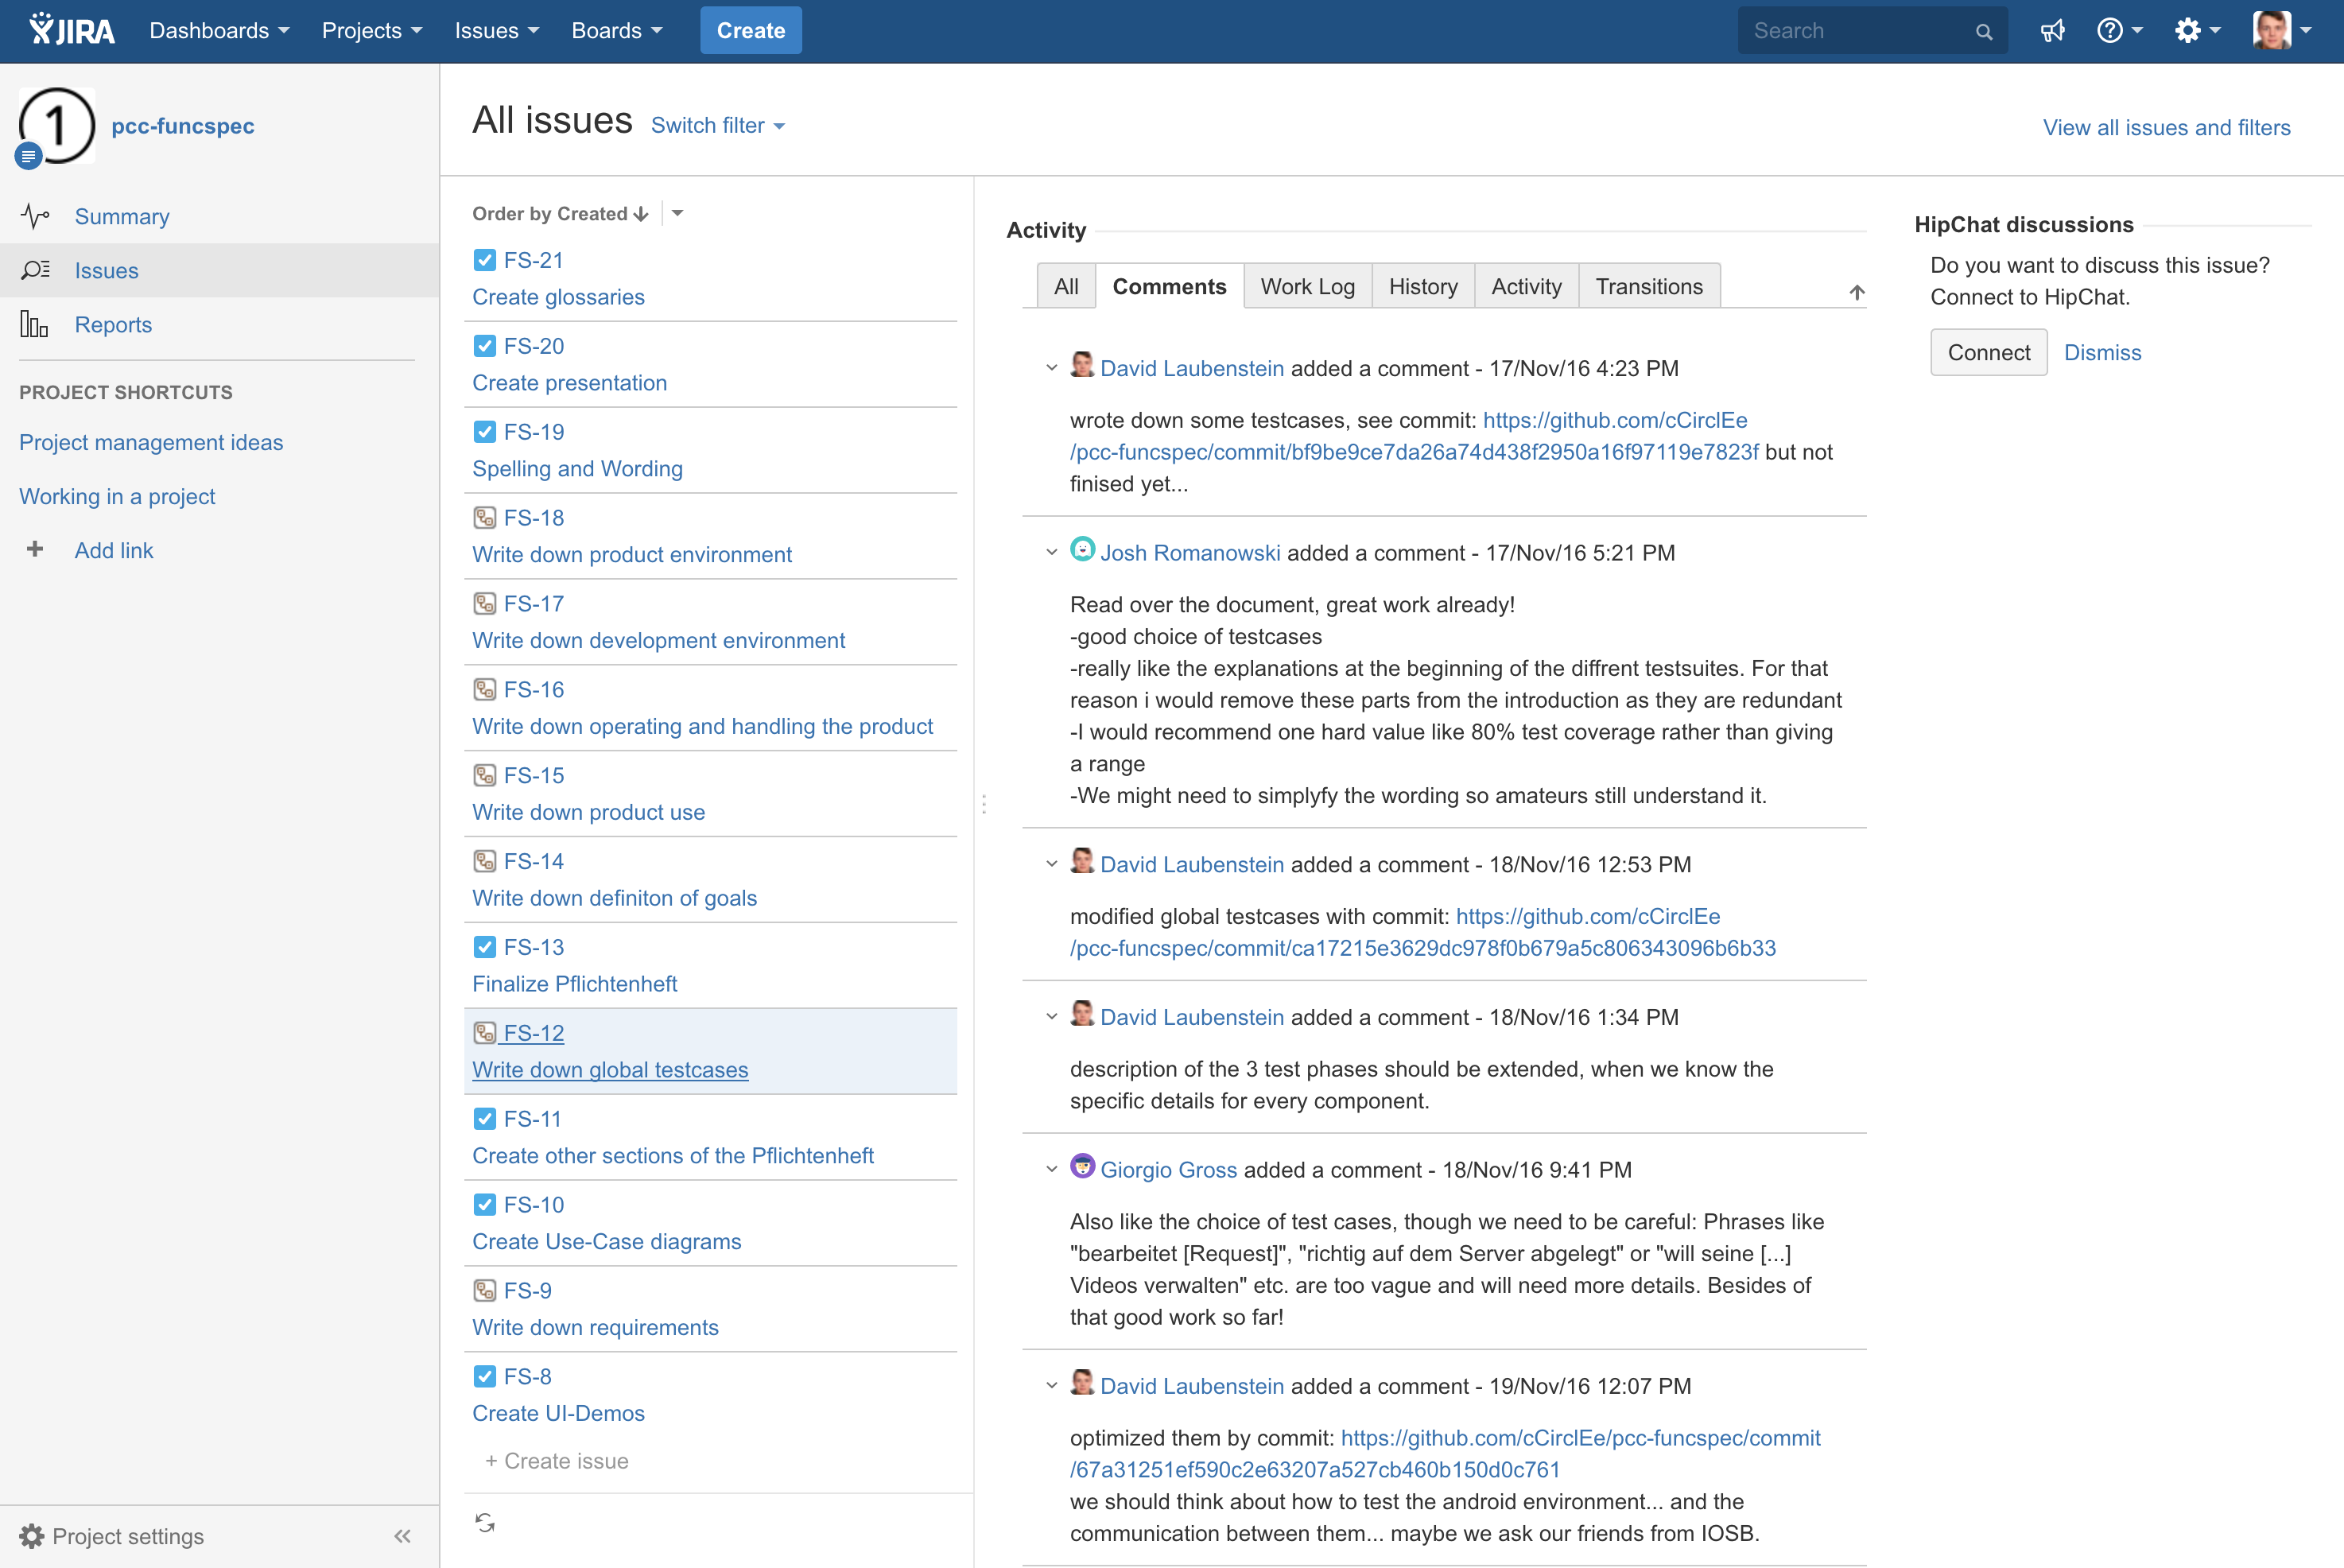
\includegraphics[scale=0.18]{logos/JIRA02} 
		\end{center}
	\end{figure}				
\end{frame}

\subsection{Github}
\begin{frame}[allowframebreaks]{Github}
	\begin{figure}
		\begin{center}
			%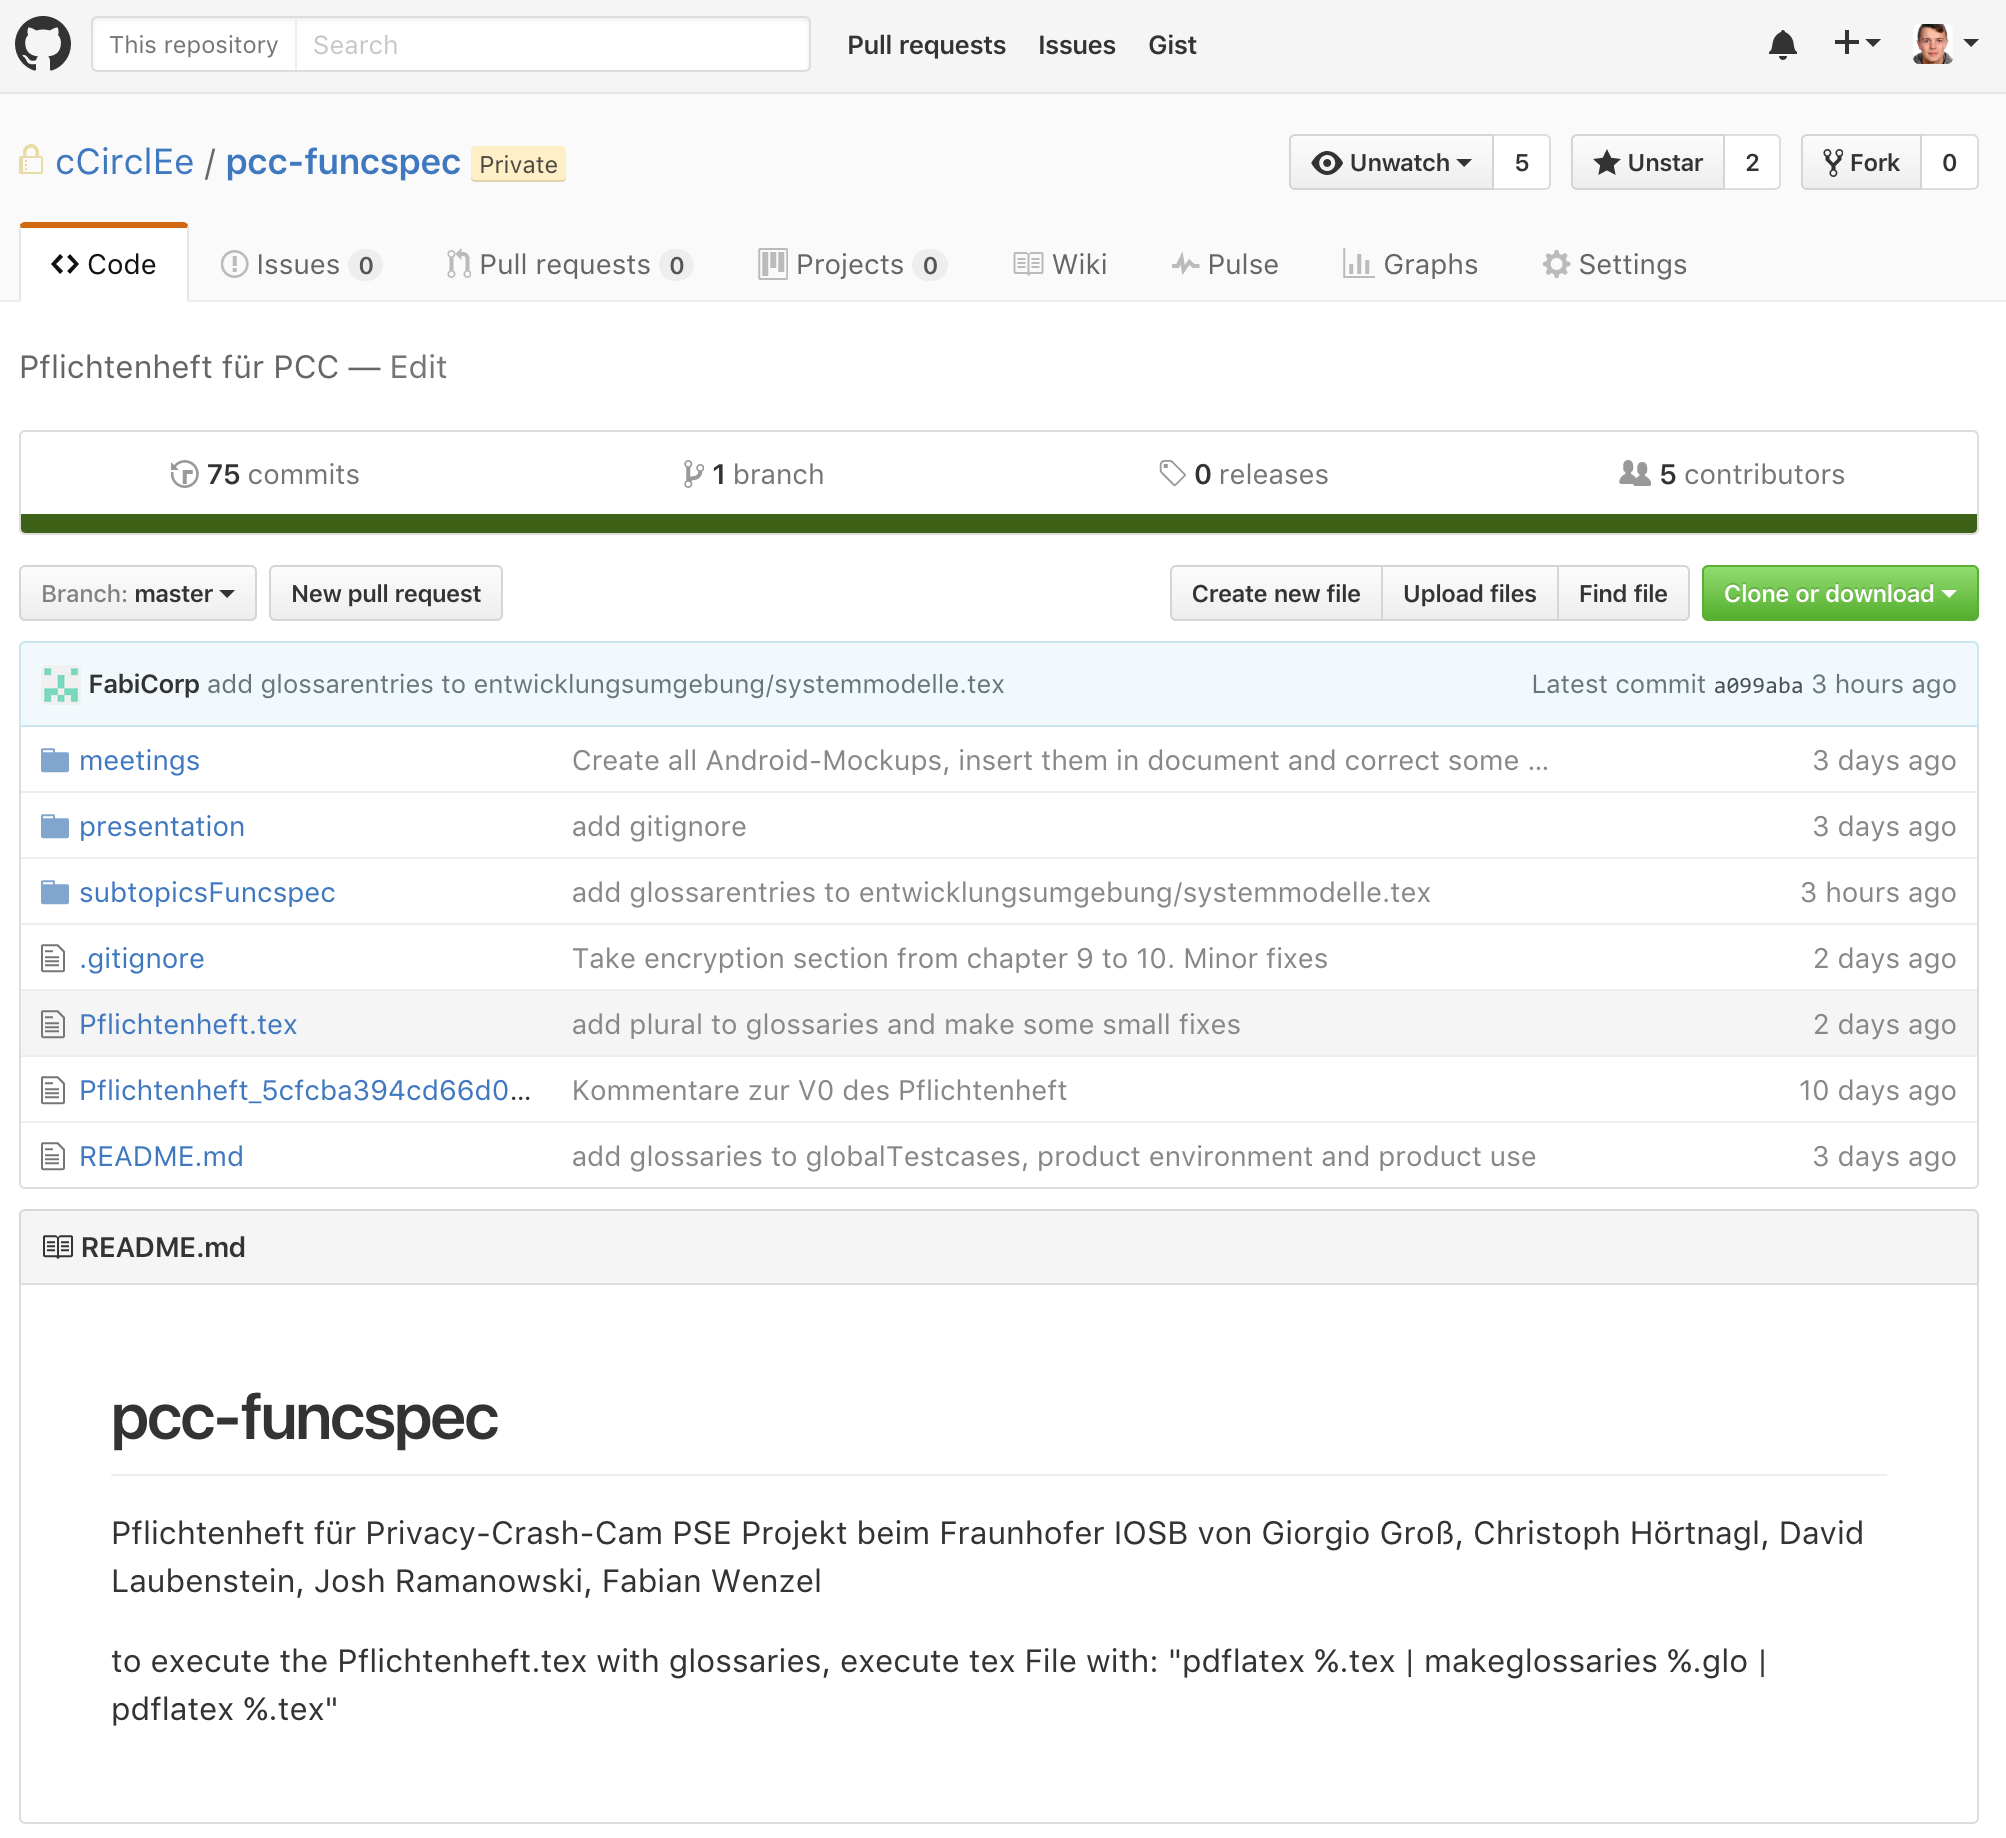
\includegraphics[scale=0.20]{logos/Github} 
		\end{center}
		\framebreak
		\begin{center}
			%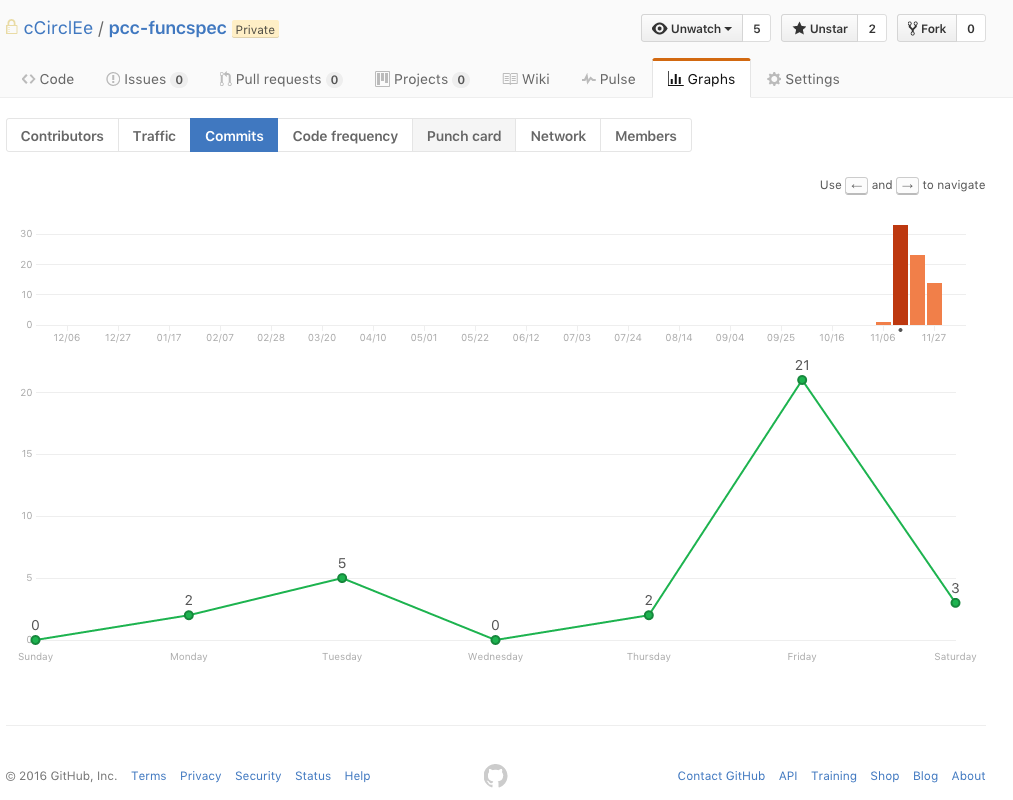
\includegraphics[scale=0.23]{logos/GithubStats} 
		\end{center}
	\end{figure}				
\end{frame}

\section{Gruppenarbeit}
\begin{frame}{Gruppenarbeit}
	\begin{figure}
		\begin{center}
			%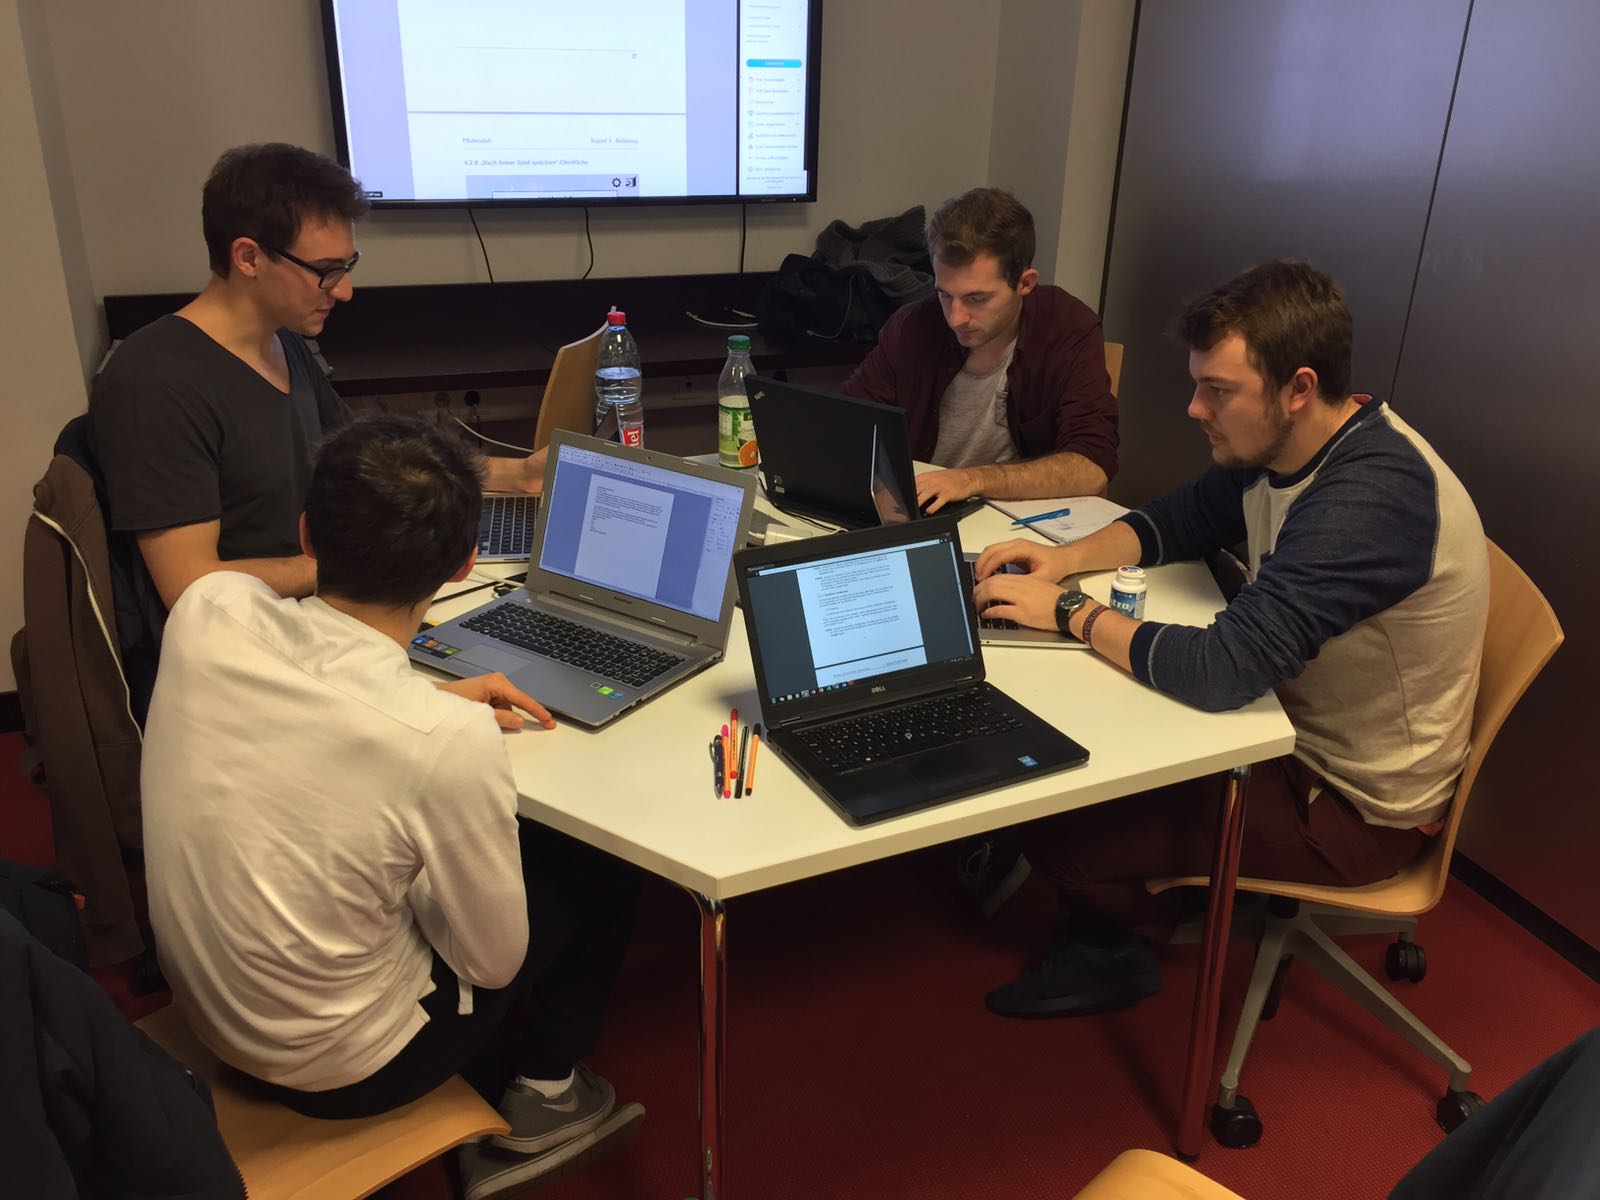
\includegraphics[scale=0.16]{logos/Gruppenarbeit} 
		\end{center}
	\end{figure}	
\end{frame}
\end{document}
